\chapter{绪论}
\enchapter{Introduction}


\section{北大西洋海洋多尺度能量串级的研究意义}
\ensection{Significance of multi-scale energy cascade in the North Atlantic Ocean}

海洋中的环流受到地球自转的影响,动能主要集中在海洋的大尺度环流,如黑潮、湾流和中尺度涡旋等空间尺度大于地转尺度的运动上。根据目前已有的卫星高度计数据,中尺度能量占据了大洋总能量的70\%以上。中尺度庞大的动能来源与去向问题一直是本世纪海洋动力学研究的热点问题。Wunsch和Ferrari在2004年回顾性的工作指出 $\cdots\cdots$ 


\section{中尺度涡旋与亚中尺度过程之间的能量串级}
\ensection{Energy cascade between mesoscale eddies and sub-mesoscale processes}

\subsection{中尺度漩涡}
\ensubsection{Mesoscale eddy}

中尺度涡旋在海洋中广泛存在,其空间尺度通常在50公里-500公里,被认为是低阶近似满足地转平衡的最小尺度海洋运动过程,因此其水平运动远远大于垂直运动,具有较小罗斯贝数和较大理查德森数。中尺度涡旋较为稳定,周期从几天到数月。

\subsection{亚中尺度漩涡}
\ensubsection{Submesoscale eddy}

亚中尺度指从中尺度到耗散尺度之间这一宽阔尺度的粗略划分。在这部分中存在涡旋、锋面以及涡丝等多种运动形式。从NASA的MODIS卫星观测的表面叶绿素为亚中尺度涡丝和锋面频繁出现提供了证据[2]。除此之外,部分亚中尺度涡旋被发现存在于上层海洋内部和海底。亚中尺度过程的周期一般为几小时到几天[3]。其空间尺度一般小于当地的罗斯

\subsection{亚中尺度与中尺度之间的能量串级}
\ensubsection{Energy cascade between submesoscale and mesoscale}


由于海洋中尺度和亚中尺度相互作用中存在着大量非线性过程,因此现有研究多引入湍流理论来解释上述过程的物理机制,称为地转湍流理论。本文对地转湍流理论的讨论分为能量注入尺度和能量串级两部分。能量注入尺度指代湍流动力学含能区的观点,即能量从该尺度进入动能谱,本文中对应不稳定发生势能转化为动能的特征尺度。能量串级概念来源于前苏联科学家Kolmogorov在谱方法基础上针对湍流研究的奠基性的工作,指能量跨尺度转移过程$\cdots\cdots$

{\color{red}``下面是一个图片的示例,进行了修改,图片标题包括英文标题和中文标题,字体为5号,居中。"}

\begin{figure}[htbp]
    \centering
    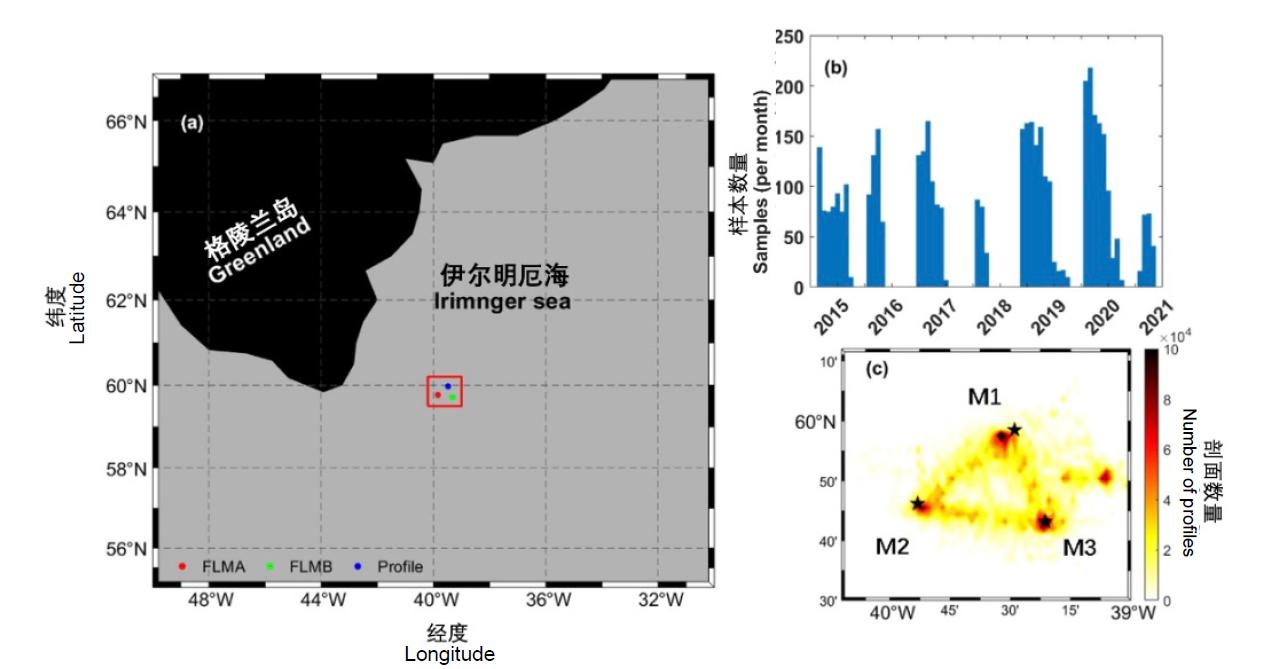
\includegraphics[width=0.8\linewidth]{img/fig_1_1_study_area.jpg}
    \figurecaption{(a) OOI项目位置,红框表示研究区域,彩色的点表示系泊。(b) 抽样概况的时间分布。(c) 采样点的空间分布,黑色的星星表示(a)中的系泊浮标}{(a) Position of OOI program, red box represents the study region, colored points indicate moorings. (b) Time distribution of sampling profiles. (c) Spatial distribution of sampling points, the blacks stars indicate the moorings in (a)}
    \label{fig:enter-label}
\end{figure}

\begin{figure}[htbp]
    \centering
    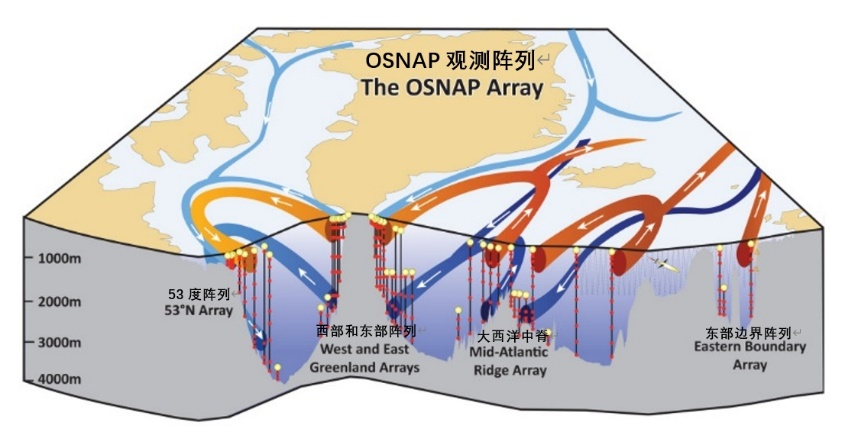
\includegraphics[width=0.5\linewidth]{img/fig_1_2_OSNAP.jpg}
    \figurecaption{北大西洋副极地翻转环流观测项目(OSNAP)阵列观测点(黄色点)空间分布}{Spatial distributions of OSNAP array observations (yellow dots)}
    \label{fig:enter-label}
\end{figure}

{\color{red}``图序采用阿拉伯数字分章编号,如第3章第2个图的图序为“图3-2”;英文标题,以Fig. 1-1编号。全文编号方式应统一。"}

\section{本章小结}
\ensection{Summary of this chapter}

前文中,我们回顾了中尺度涡旋、亚中尺度运动和近惯性内波以及它们之间的相互作用关系,然而前任工作对上述物理过程的研究往往是分散的,主要集中于讨论两两之间的相互作用,且具有时间或空间上的依赖性的,导致不同物理过程之间的相互作用的研究工作很难整合到一起$\cdots\cdots$